\documentclass{article}
%\documentclass[journal]{IEEEtran}
%\documentclass{report}
%\documentclass{acta}
\usepackage[english,polish]{babel}
\usepackage{polski}
\usepackage{graphicx}
\usepackage[utf8]{inputenc}

\usepackage{courier}

\usepackage{listings}
\lstloadlanguages{TeX}

\lstset{
	literate={ą}{{\k{a}}}1
           {ć}{{\'c}}1
           {ę}{{\k{e}}}1
           {ó}{{\'o}}1
           {ń}{{\'n}}1
           {ł}{{\l{}}}1
           {ś}{{\'s}}1
           {ź}{{\'z}}1
           {ż}{{\.z}}1
           {Ą}{{\k{A}}}1
           {Ć}{{\'C}}1
           {Ę}{{\k{E}}}1
           {Ó}{{\'O}}1
           {Ń}{{\'N}}1
           {Ł}{{\L{}}}1
           {Ś}{{\'S}}1
           {Ź}{{\'Z}}1
           {Ż}{{\.Z}}1,
	basicstyle=\footnotesize\ttfamily,
}

% ------------------------
\begin{document}

\title{Przedstawienie optymalizacji wyznaczania sąsiedztwa}
\author{mgr inż. Tomasz Gajda, mgr inż. Jakub Porzycki}

\maketitle

\begin{abstract}
Przedstawienie optymalizacji wyznaczania sąsiedztwa w modelu Social-Force wraz z doborem optymalnych parametrów.

\end{abstract}


\section{Wprowadzenie}

Najbardziej wymagającym obliczeniowo elementem symulacji korzystającym z modelu Social-Force jest wyznaczenie najbliższego sąsiedztwa. Aby tego dokonać trzeba sprawdzić odległości pomiędzy każdą parą pieszych co przy kwadratowej złożoności oraz tłumach liczących tysiące osób istotnie spowalnia obliczenia.
Aby zniwelować liczbę obliczeń konieczne było wprowadzenie nowej fazy obliczeń która wstępnie odrzuci pieszych znajdujących się zbyt daleko. 
Zaproponowane rozwiązanie będzie polegać na podziale przestrzeni (Space partitioning), często stosowanym w grach komputerowych przy wykrywaniu kolizji. Polega on na podziale przestrzeni na obszary (najczęściej kwadraty) do których przypisani zostaną piesi na podstawie pozycji. W bardziej złożonych przypadkach możliwe jest stosowanie hierarchicznego podziału w zależności od gęstości, tutaj jednak zostanie omówiony przypadek o prostej strukturze.  

\section{Opis}
W modelu Social-Force siłą separacji, która wymaga wyznaczenia najbliższego sąsiedztwa posiada parametr odcięcia określa promień, w którym na pieszego oddziaływają inni piesi. Parametr pozwala nam wyznaczyć ilość sąsiednich obszarów oraz ich optymalny rozmiar. Na podstawie wybranych obszarów tworzona jest lista potencjalnych sąsiadów którzy znajdują się w pobliskich obszarach.

Efektywność tego algorytmu jest silnie uzależniona od rozmiaru siatki. Za duży sprowadzi się do stanu podstawowego w którym porównujemy każdą z par, za mały wprowadzi duży narzut przy obsłudze łączenia list pieszych.


\begin{figure}
    \centering
    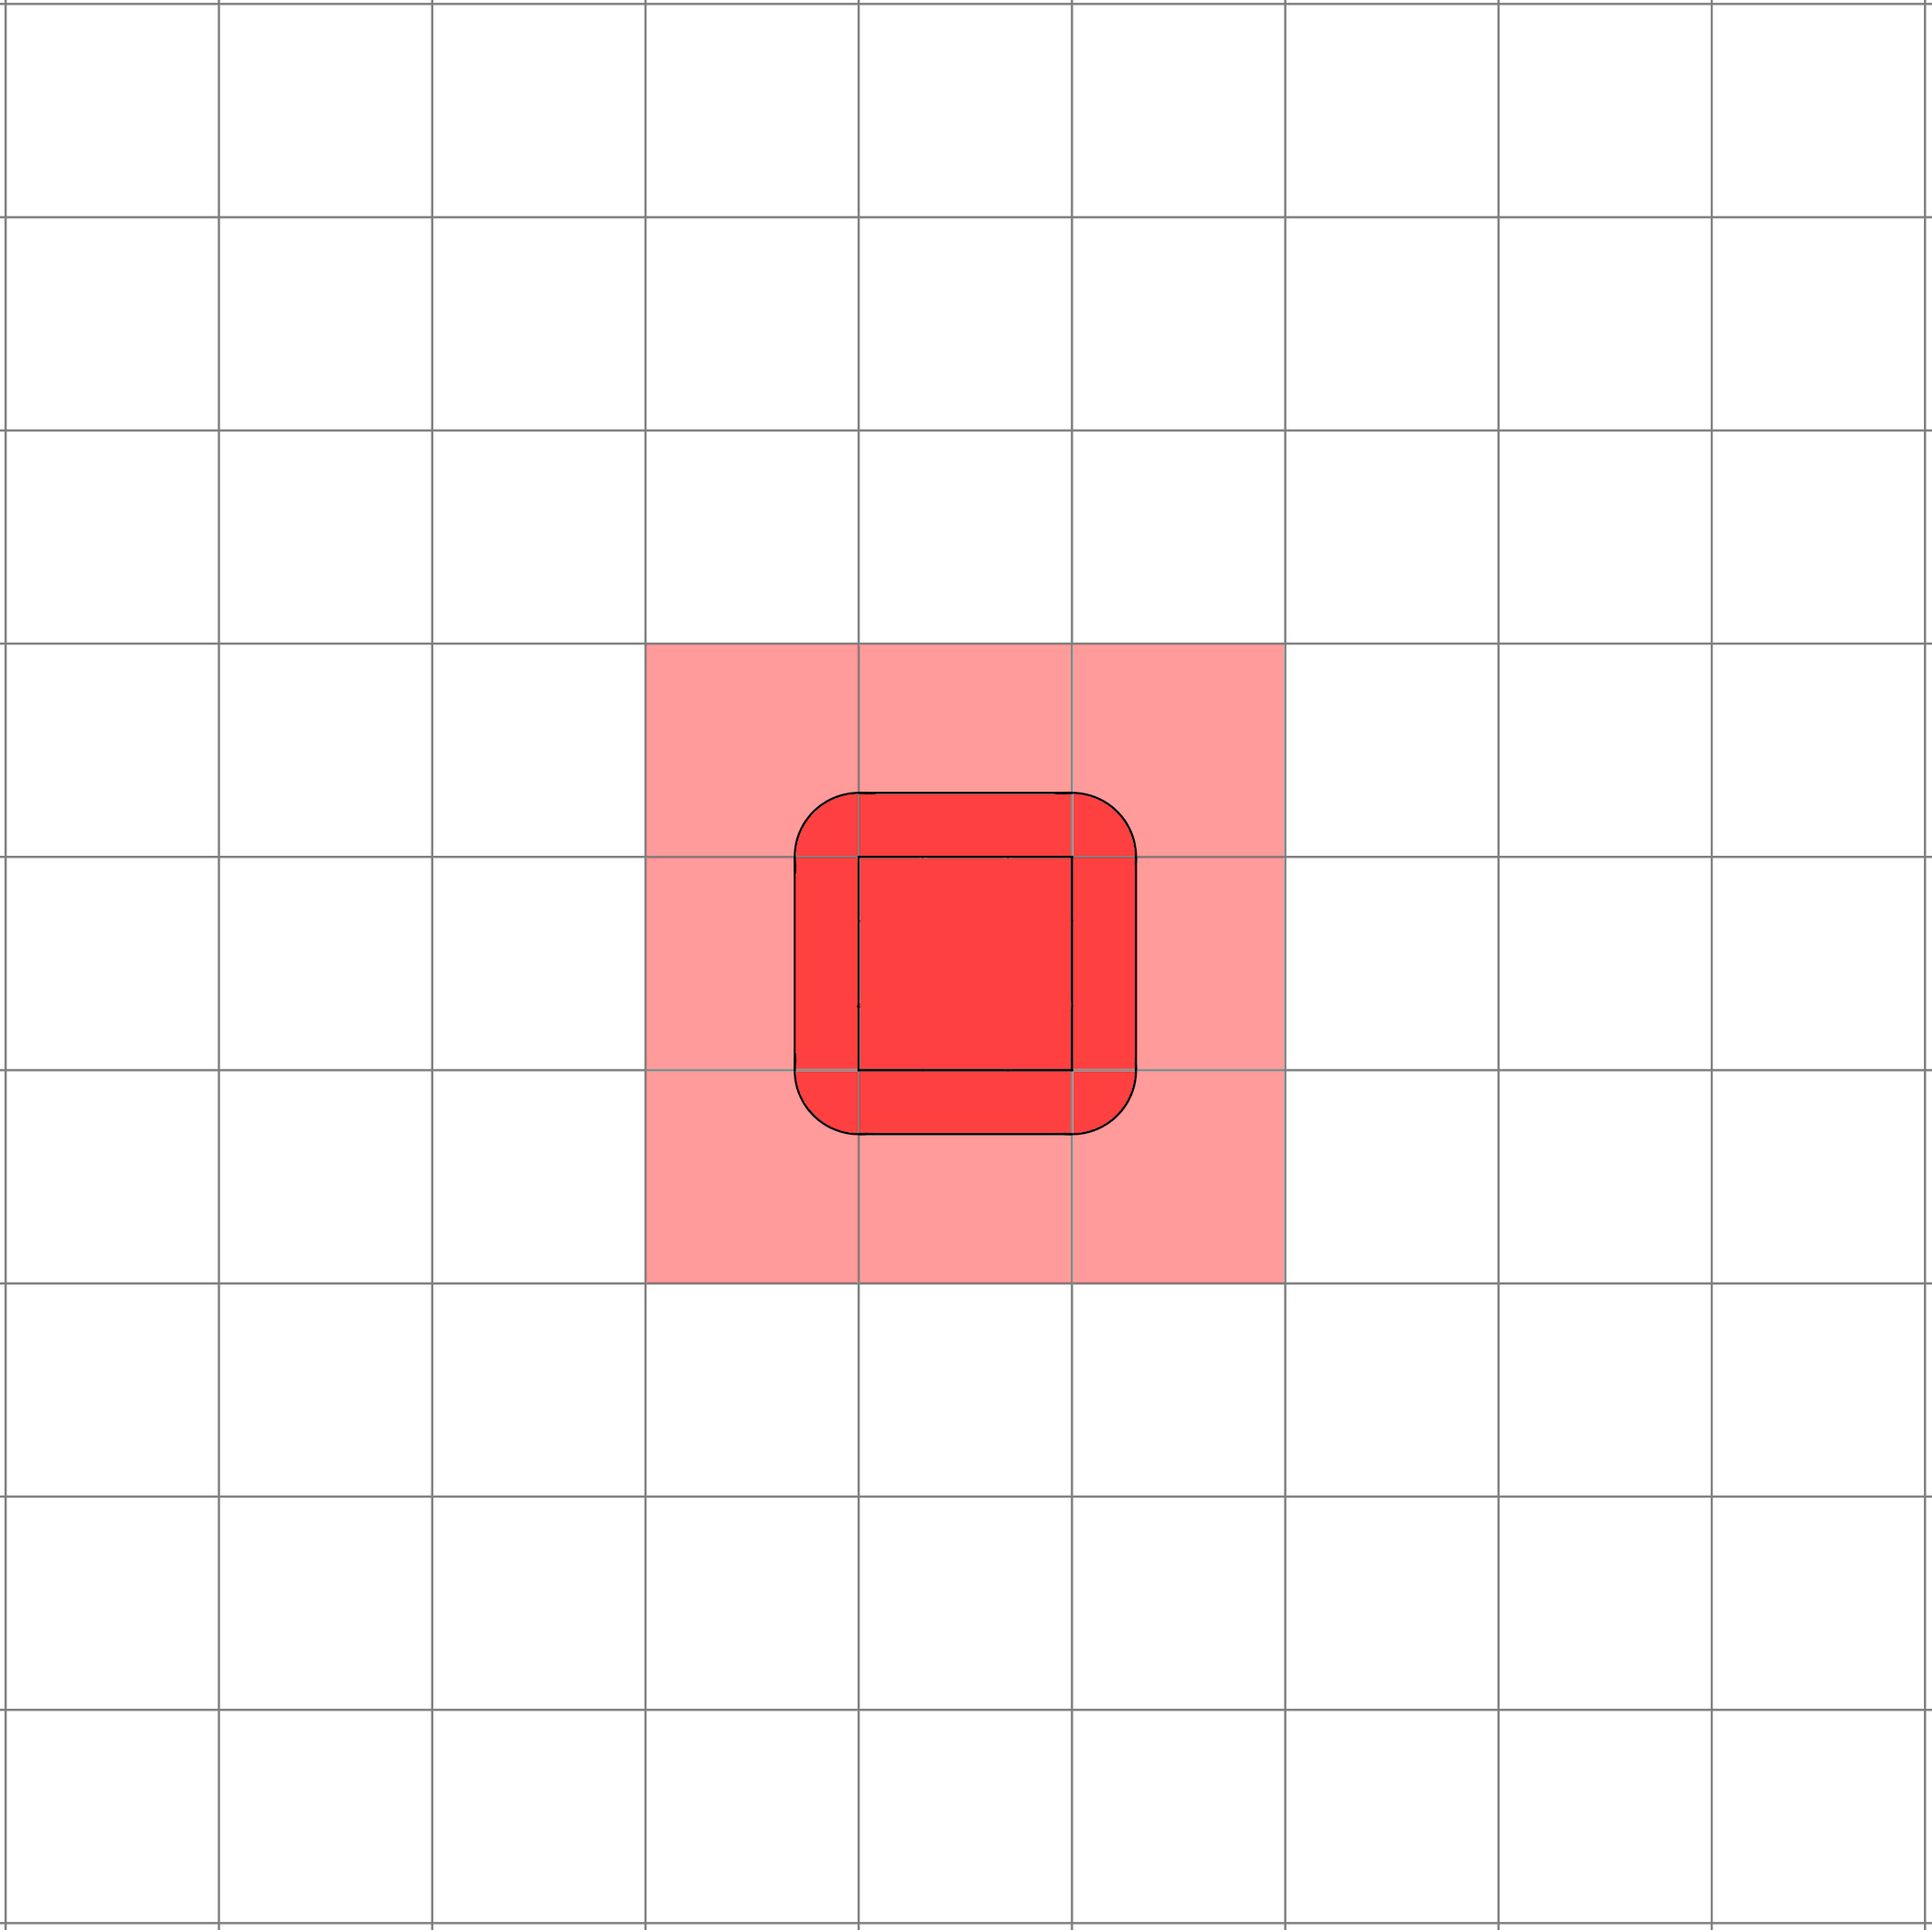
\includegraphics[width=2.5in]{0,3.png}
    \caption{Przykładowe działanie dla małego promianie odcięcia (ciemny czerwony potencjalny zasięg widzenia, jasny czerwony badane komórki obszaru)}
    \label{rys:ex_1}
\end{figure}

\begin{figure}
    \centering
    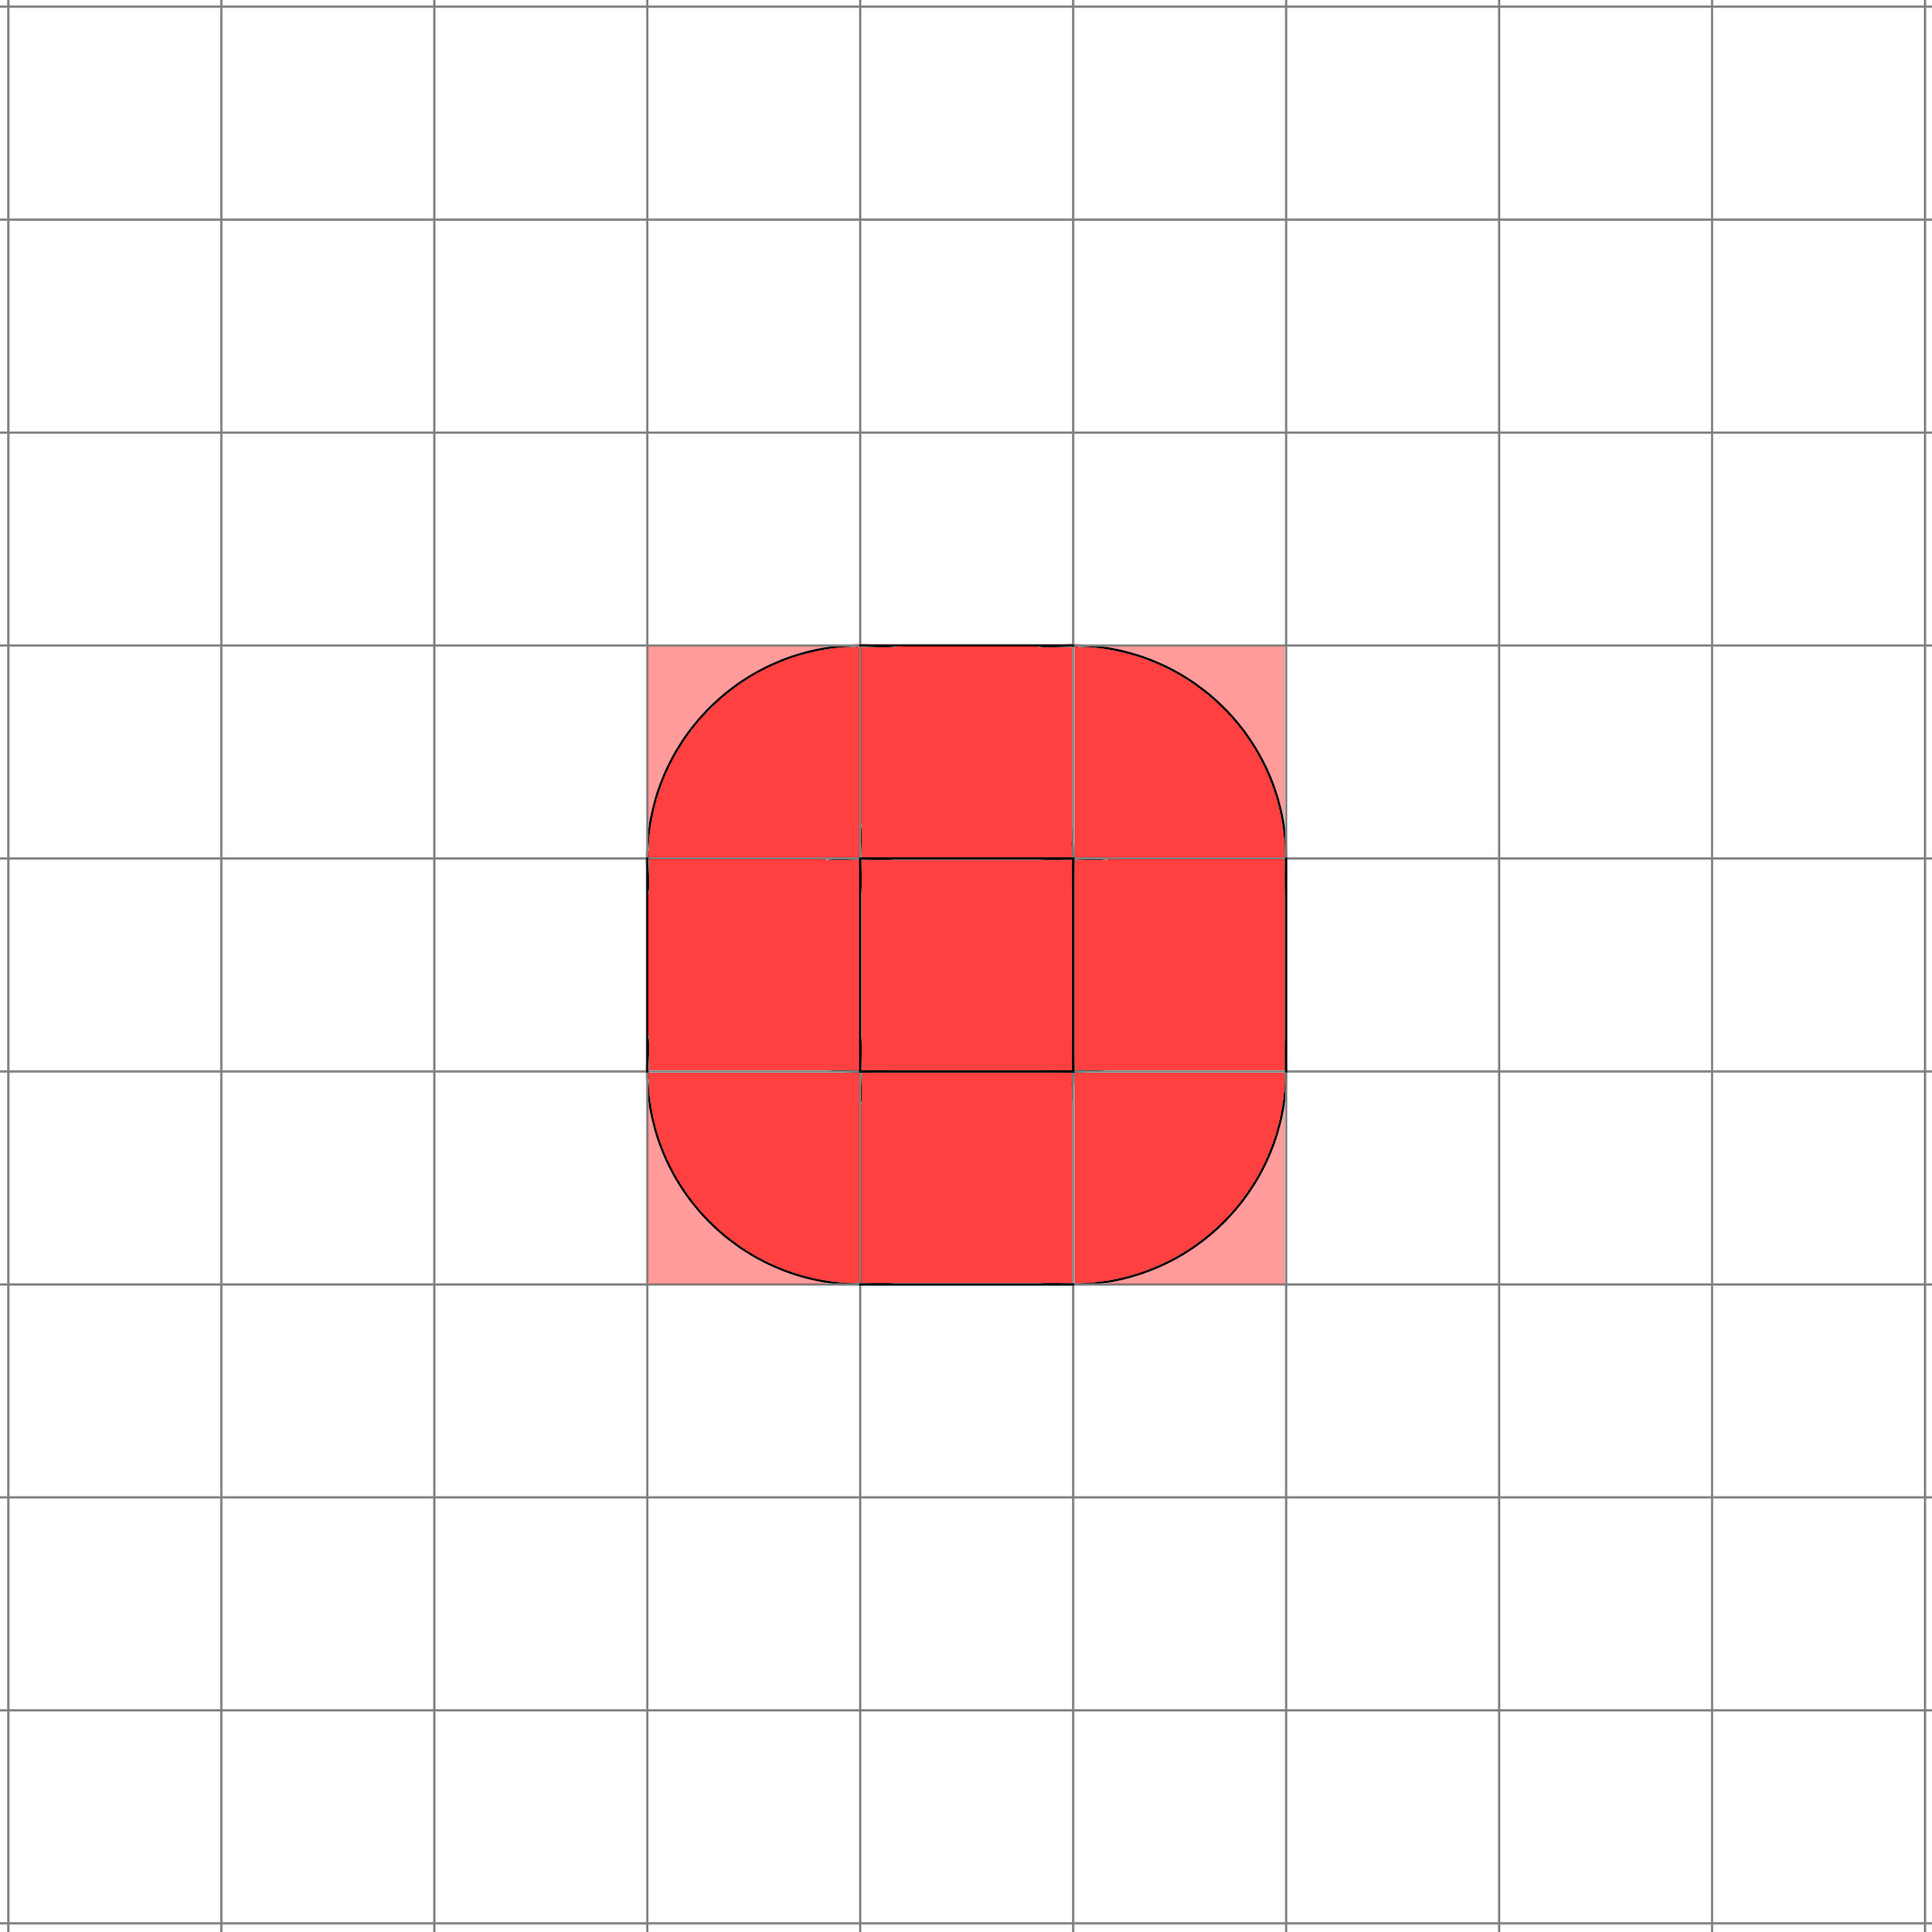
\includegraphics[width=2.5in]{1.png}
    \caption{Przykładowe działanie dla średniego promianie odcięcia (ciemny czerwony potencjalny zasięg widzenia, jasny czerwony badane komórki obszaru)}
    \label{rys:ex_2}
\end{figure}

\begin{figure}
    \centering
    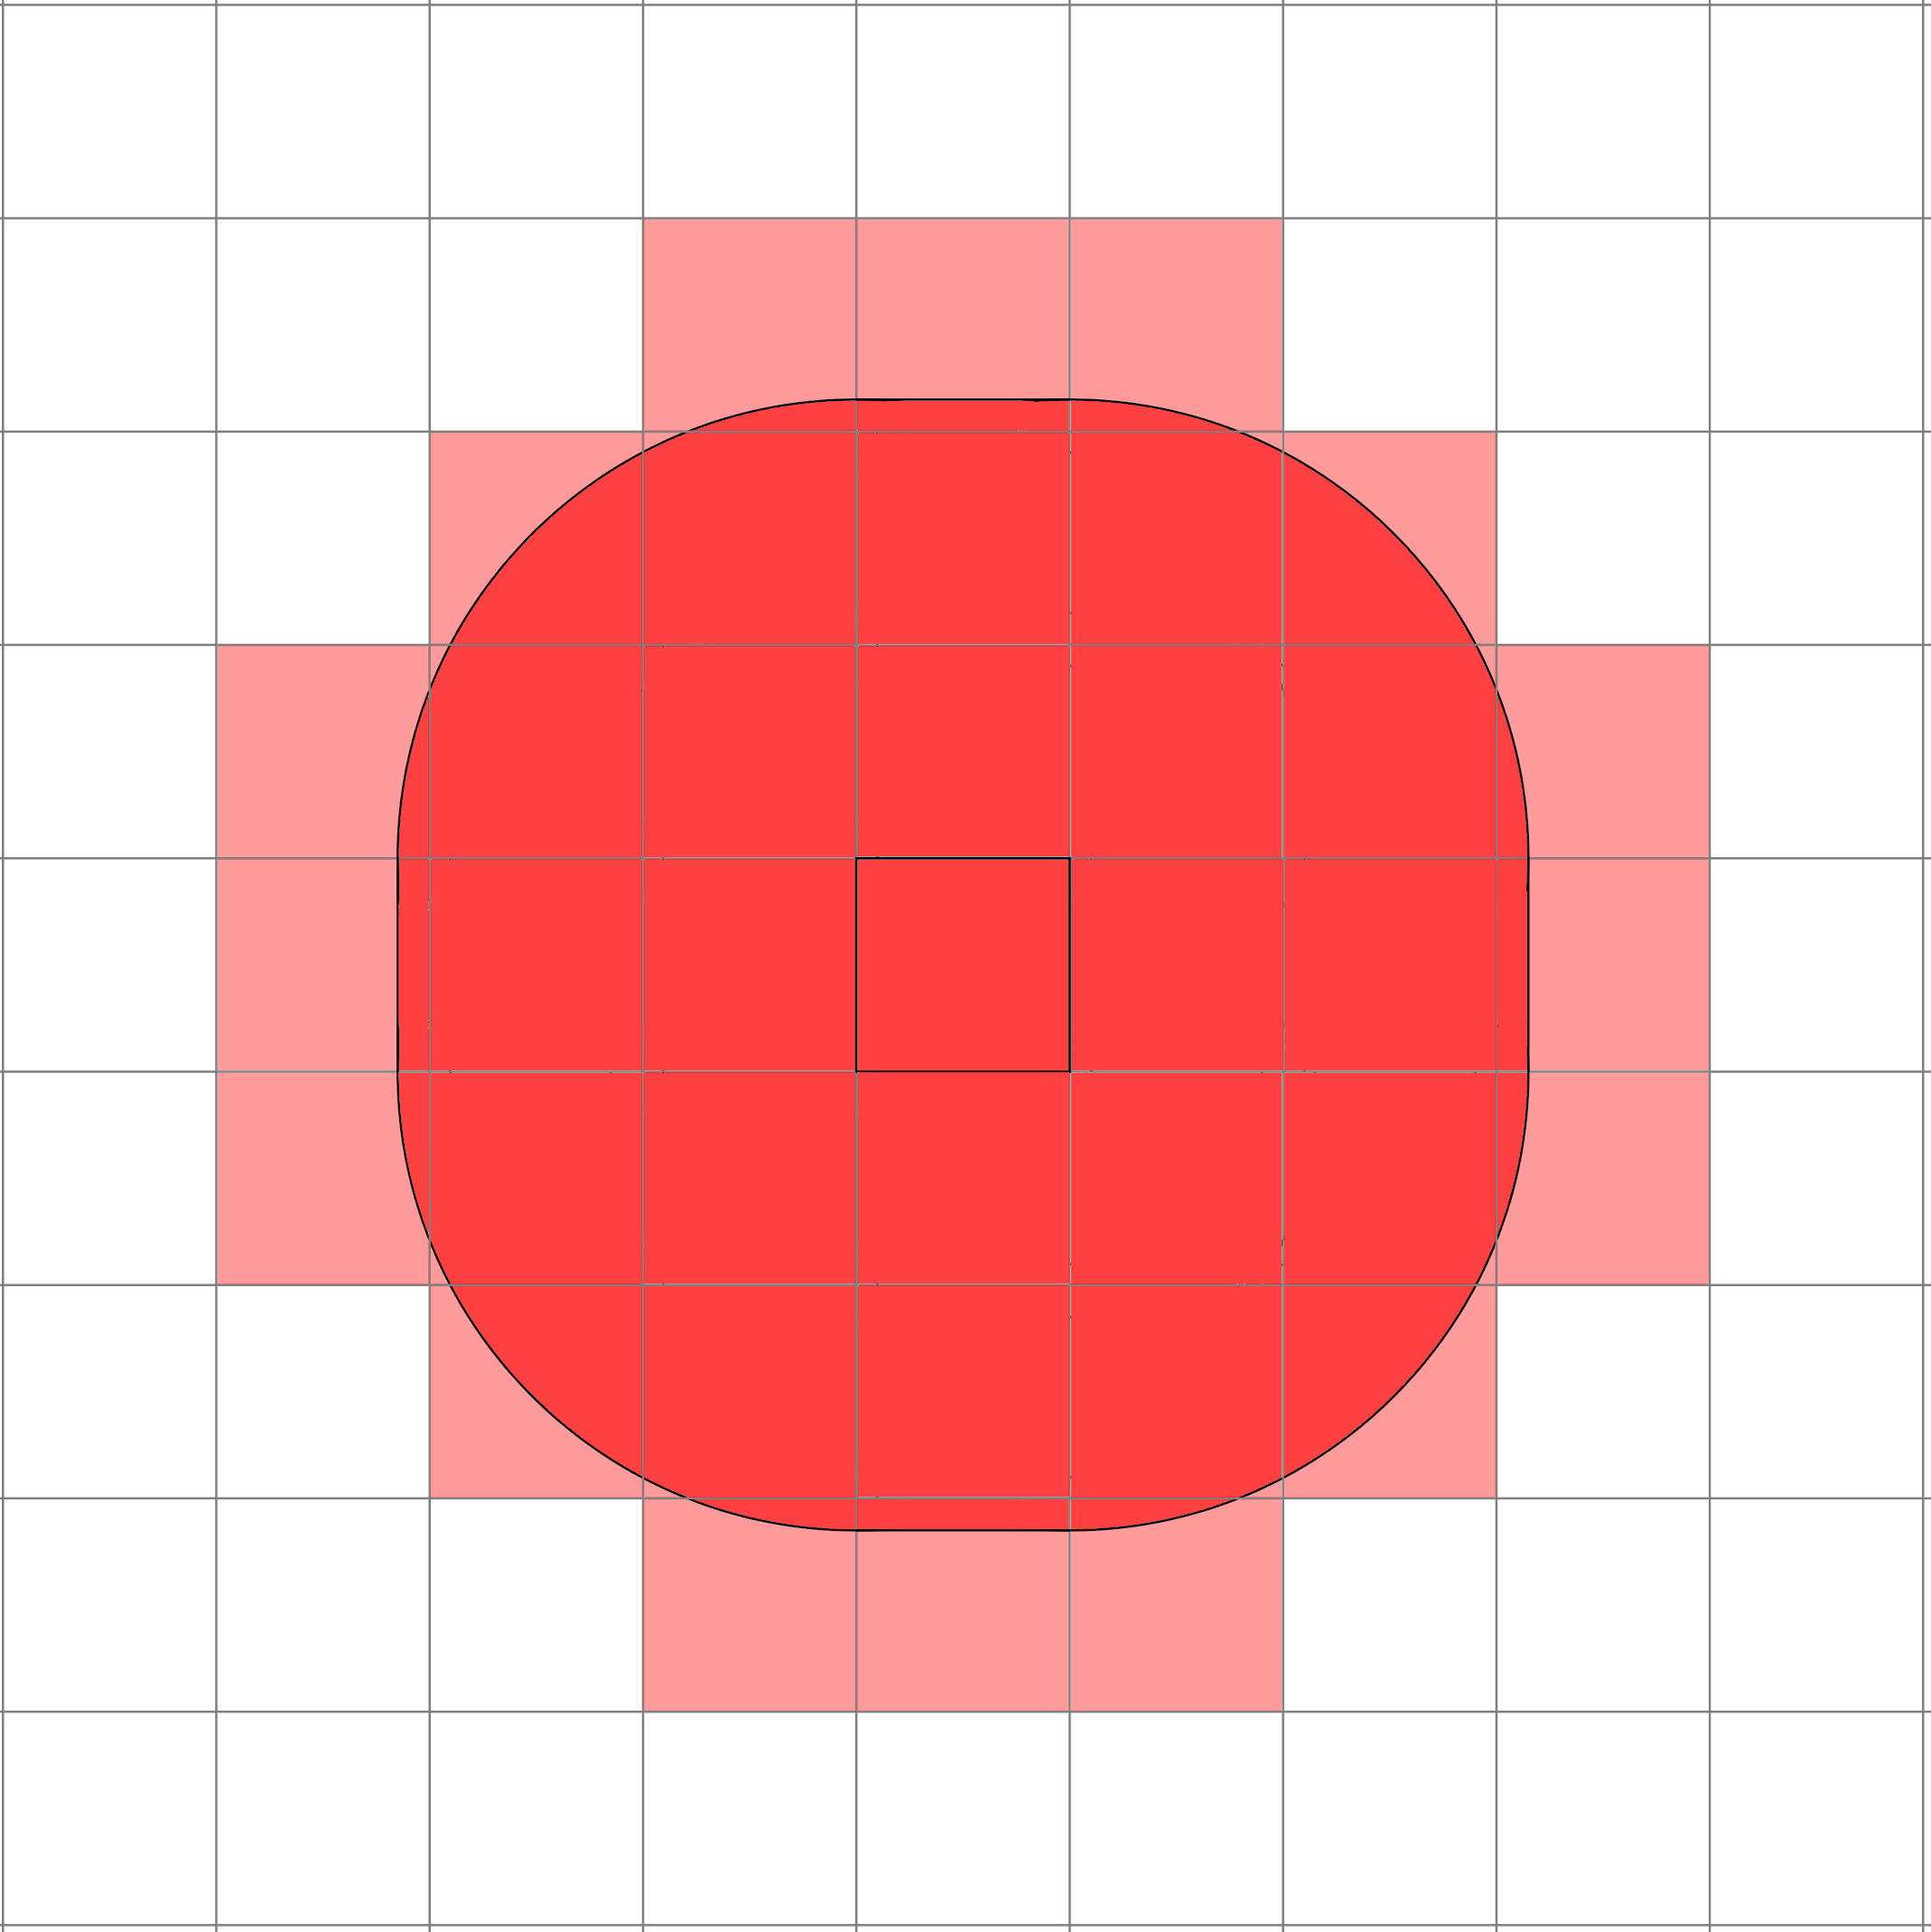
\includegraphics[width=2.5in]{2,15.png}
    \caption{Przykładowe działanie dla dużego promianie odcięcia (ciemny czerwony potencjalny zasięg widzenia, jasny czerwony badane komórki obszaru)}
    \label{rys:ex_3}
\end{figure}

\section{Testy}
Testy zostały przprowadzone dla modelu bez optymalizacji oraz dla wersji zoptymalizowanej dla różnych wielkości obszarów. Promień odcięcia został ustalony na wartość 2. W testach wyłączono pozstałe siły aby wyniki jak najlepiej pokazywały optymalizację. Wyniki przedstawiono jako średnią czasu jaki był potrzebny na obliczenie jednego kroku symulacji ze średniej zostały wykluczone 10\% największych i najmniejszych wartości. Początkowa gęstość niezależnie od ilości pieszych była stała.

\begin{figure}
    \centering
    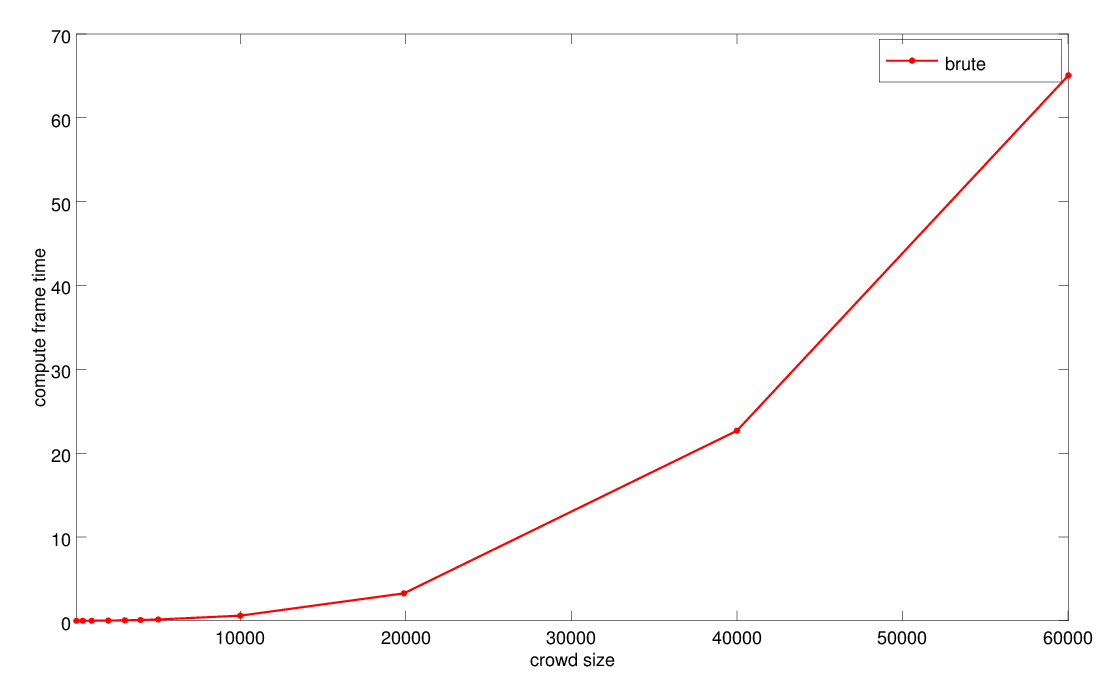
\includegraphics[width=5.5in]{onlyBrute.png}
    \caption{Wyniki dla metody podstawowej}
    \label{rys:result1}
\end{figure}

\begin{figure}
    \centering
    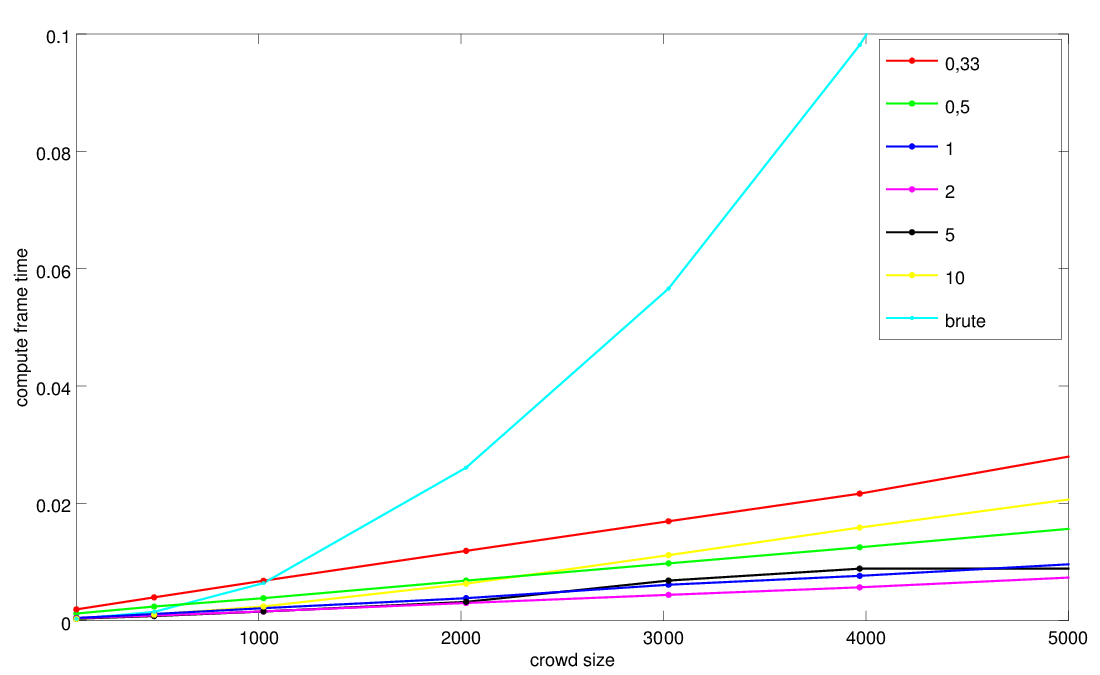
\includegraphics[width=5.5in]{both5000.png}
    \caption{Porównanie do 5000 pieszych}
    \label{rys:result2}
\end{figure}

\begin{figure}
    \centering
    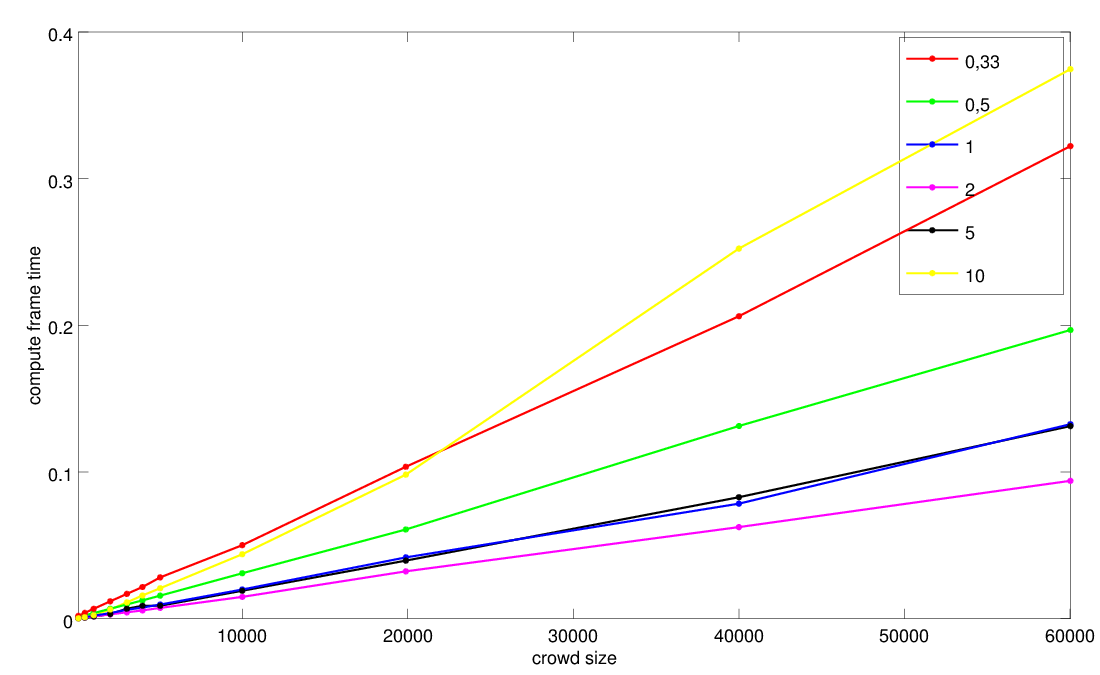
\includegraphics[width=5.5in]{optimizeAll.png}
    \caption{Porównanie tylko wersji zoptymalizowanych}
    \label{rys:result3}
\end{figure}

\begin{figure}
    \centering
    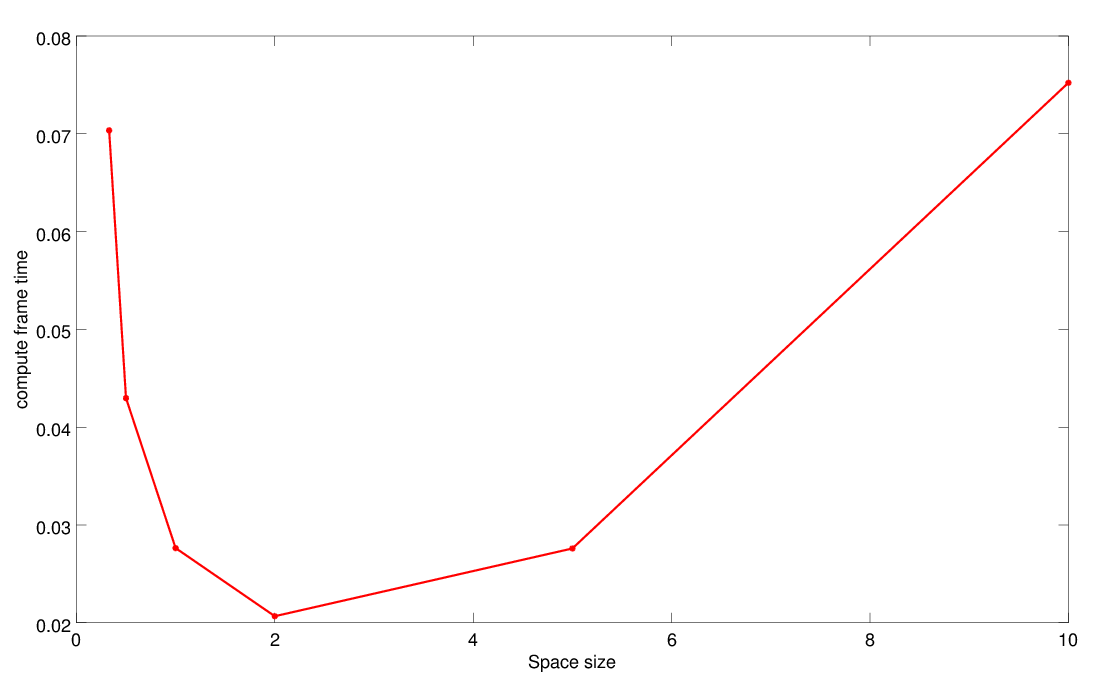
\includegraphics[width=5.5in]{spaceSize.png}
    \caption{Porównanie średniej wydajności w zalżności od rozmiaru obszaru}
    \label{rys:result4}
\end{figure}

\section{Wnioski}

Z wykonanych testów wyraźnie widać zmniejszenie narzutu wydajnościowego w zoptymalizowanej metodzie. Tylko przy bardzo małych wartościach do 300 metoda podstawowa jest wydajniejsza. Wraz ze wzrostem przewaga metody z podziałem przestrzeni zwiększa się w szybkim tempie. Zgodnie z intuicją najlepszym rozmiarem, na który trzeba podzielić obszar symulacji jest rozmiar równy promieniowi odcięcia. Pozawala on na rozpatrywanie tylko dziewięciu obszarów, co zapobiega wielu operacji łączenia list pieszych (w wersji zoptymalizowanej jest to najbardziej kosztowna operacja). Jednocześnie minimalizowany jest obszar, który jest sprawdzany, mimo iż jest za daleko (obszar jasno czerwony na rysunku \ref{rys:ex_2})

 Wyniki metody podstawowej można aproksymować wzorem \ref{eq:perf_basic} ze współczynnikiem determinacji  $R^{2}=0,9986$.
\begin{equation}
\label{eq:perf_basic}
 y=2\cdot 10^{-8}n^{2}+4\cdot 10^{-4}n+0,7913
\end{equation}
gdzie $n$ - liczba pieszych

Wyniki dla najlepiej dobranego rozmiaru obszaru wynoszącego 2 tyle, co promień odcięcia, można aproksymować wzorem \ref{eq:perf_optm} ze współczynnikiem determinacji  $R^{2}=0,9997$.
\begin{equation}
\label{eq:perf_optm}
 y=2\cdot 10^{-6}n+-0,0001
\end{equation}
gdzie $n$ - liczba pieszych

\end{document}
